\begin{figure}%[tbp]
	\begin{subfigure}[b]{.45\textwidth}
	\centering
	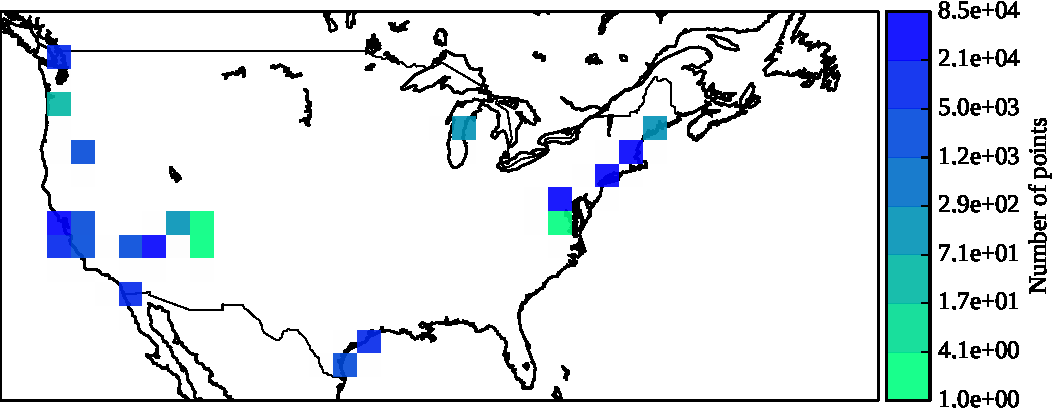
\includegraphics[width=\textwidth]{pix/freq_COM_usa_coast.pdf}
		%\caption{Frequency plot}
		%\label{fig:gull}
	\end{subfigure}
	\hfill
	\begin{subfigure}[b]{.45\textwidth}
	\centering
	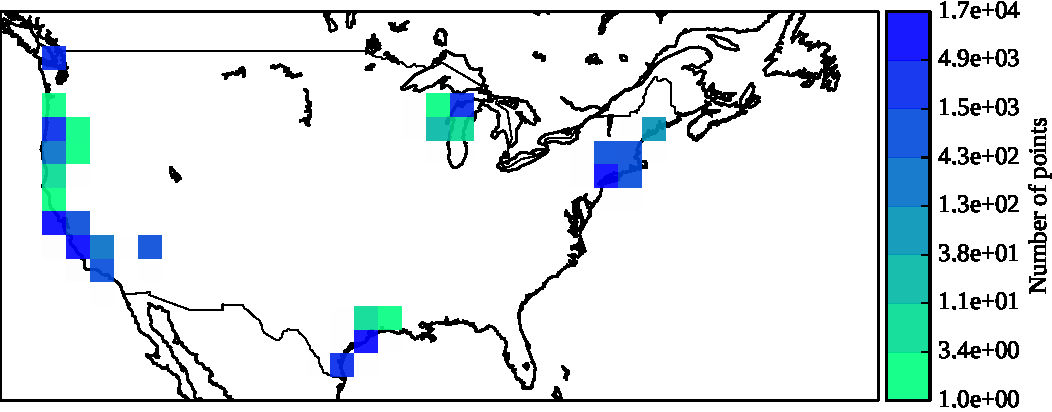
\includegraphics[width=\textwidth]{pix/freq_RW_usa_coast.pdf}
		%\caption{coast}
		%\label{fig:gull}
	\end{subfigure}
	\,
	\begin{subfigure}[b]{.45\textwidth}
	\centering
	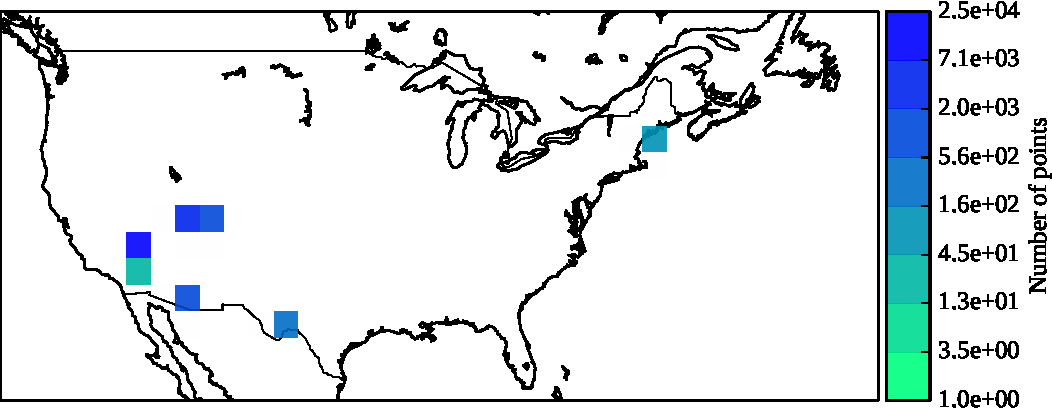
\includegraphics[width=\textwidth]{pix/freq_COM_usa_desert.pdf}
		%\caption{Frequency plot}
		%\label{fig:gull}
	\end{subfigure}
	\hfill
	\begin{subfigure}[b]{.45\textwidth}
	\centering
	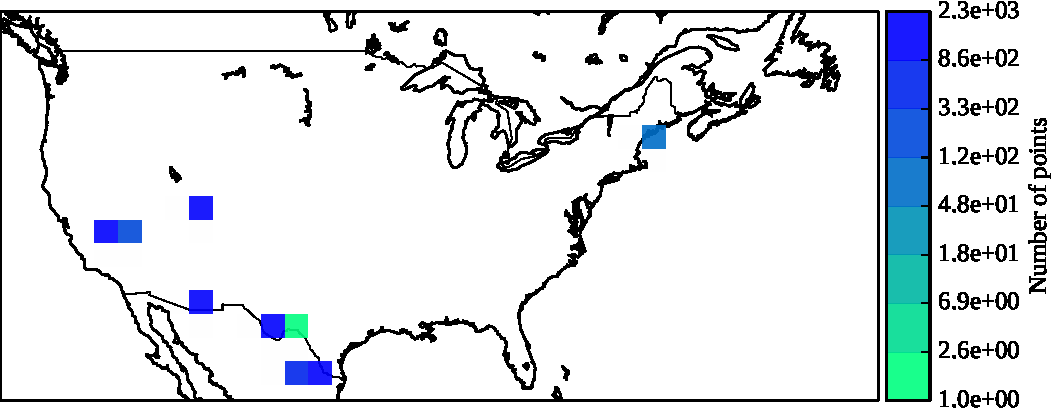
\includegraphics[width=\textwidth]{pix/freq_RW_usa_desert.pdf}
		%\caption{desert}
		%\label{fig:gull}
	\end{subfigure}
	\,
	\begin{subfigure}[b]{.45\textwidth}
	\centering
	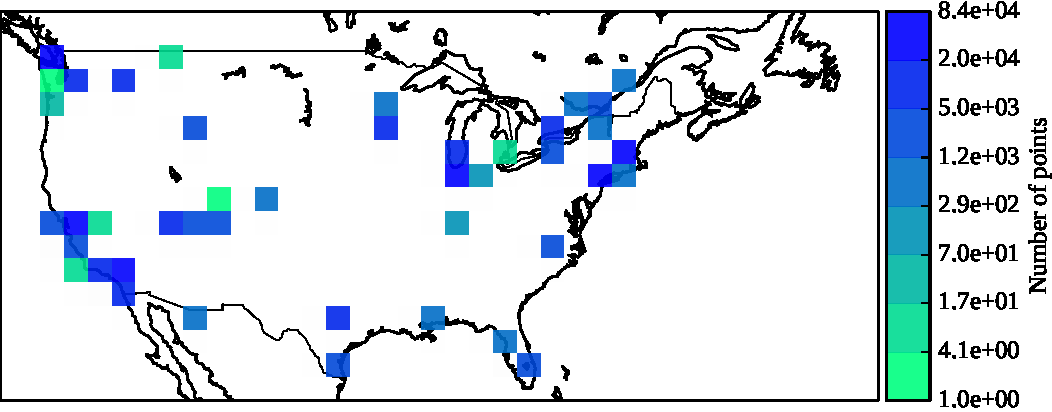
\includegraphics[width=\textwidth]{pix/freq_COM_usa_nature.pdf}
		\caption{CM}
		%\label{fig:gull}
	\end{subfigure}
	\hfill
	\begin{subfigure}[b]{.45\textwidth}
	\centering
	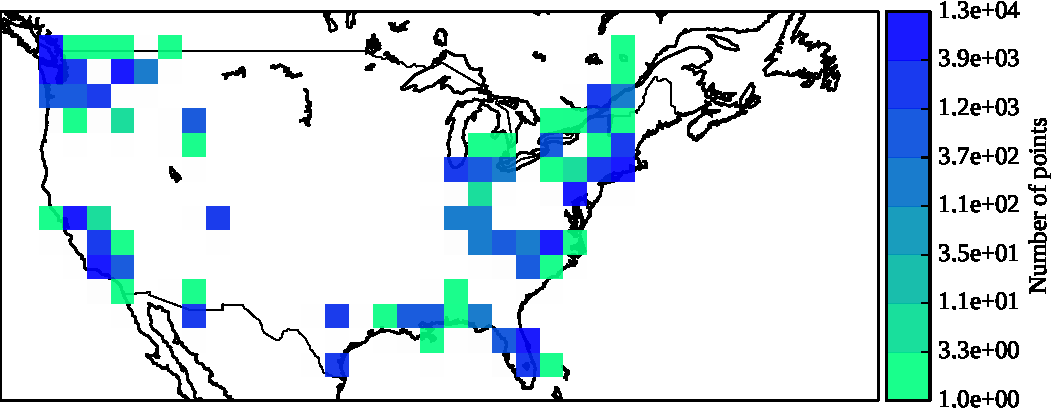
\includegraphics[width=\textwidth]{pix/freq_RW_usa_nature.pdf}
		\caption{GM}
		%\label{fig:gull}
	\end{subfigure}
	%
	\caption[Distributions for \emph{coast}, \emph{desert}, \emph{nature} with dataset C.]{The first column contains the plots for the combined metric and the second for the graph metric. The first row shows the distributions for \emph{coast}, the second for \emph{desert} and the third for \emph{nature}.}
	\label{fig:C_comp}
\end{figure}